\clearpage
 \section{Implementation details}
\subsection{Software design}
$DIYABC$ v2 has been designed in a very different way compared to version 1. Version 1 was a single executable file were the GUI \footnote{Graphic User Interface} and computation codes were highly intricated and both written in the same language (\emph{Delphi}). In version 2, the GUI and the computation codes have been completely separated. Actually, the GUI is a script written in \emph{python} and all computations are included in a program written in \emph{C++}. In opposition to \emph{Delphi} which is restricted to a single OS (\texttt{Windows}), \textit{python} and \textit{C++} can be used with the main three OS (\texttt{Linux}, \texttt{Mac} and \texttt{Windows}), allowing version 2  to be operated under all three OS.\\
The GUI uses the \textit{Qt} graphic library. The computation code is linked to the \textit{openmp} library allowing a better use of multicore/multiprocessor computers.\\
The GUI can launch the computation program with the right parameters and keeps track of the progress of the latter through small log files. The GUI can launch as many computation programs as there are open projects, but no more than one computation program per project. A \textit{lock} file located in the project directory is created when the computation program is launched by the GUI and removed when the computation program has normally terminated. When the computation program has exited anormaly, the GUI issues an error message trying to explain where the programm failed.    
\subsection{Files}
The program uses and produces various files which we will describe now.
\subsubsection{data files}
Data files are text files that contain information about the samples : number and names of microsatellite markers, multilocus genotypes of individuals. The basic  format is that of the Genepop software \citep{RR1995} and data files produced by DIYABC are under this format.  \textbf{Microsatellite genotypes must be noted with 3 (haploid) or 6 (diploid) digits, these three digit numbers being the length in nucleotides of the corresponding PCR products}. In addition, we have added some features to this basic format in order to use sequence data. All these additions are explained in section 4.4.\\ 
Any extension is accepted for datafile names, including no extension at all. If the data file is simulated with $DIYABC$, the extension is \texttt{mss} for microsatellite/DNA sequence data and \texttt{snp} for SNP data. The next page shows examples of data sets saved.

\subsubsection{reference table files} 
Reference table files are binary files which include two successive parts :
\begin{itemize}
 \item The first part is a header which contains information necessary to read the second part, such as the number of scenarios, or the number of parameters of each scenario.
 \item The second part contains simulated data set records, each record containing the scenario number, the parameter and summary statistics values.
\end{itemize}
 
 Each time a reference table is created or increased (each time the \fbox{\textsf{Run computation}} button is pressed), a text file is created in the project directory with the name \texttt{first\_records\_of\_the\_reference\_table\_X.txt} in which \texttt{X} is an integer number starting at 0 and increasing each time the \fbox{\textsf{Run computation}} button is pressed. This file provides a text version of the first $n$ newly created records of the reference table ($n$ being equal to the \emph{Particle loop size}, see section 3.7.3).\\

\subsubsection{output files}
As already seen, DIYABC achieves different analyses : comparison of scenarios, estimation of posterior distribution of parameters, model checking,  computation of bias and mean square errors and evaluation of confidence in scenario choice. Each analysis has its own output which can be printed and saved. Graphs are saved under the chosen format and non-graphic output are saved in text files.\\

We now describe all the files produced by each type of analysis. These files are located in directories (one directory per analysis) gathered in the \texttt{analysis} subdirectory of the project directory. Below is an example of the \texttt{TOYTEST2\_2012\_9\_26-1} project directory substructure:\\

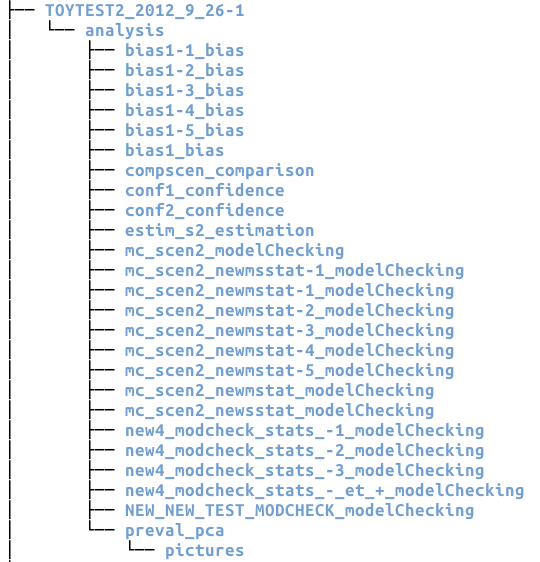
\includegraphics[scale=0.5]{gui_pictures/Capture-DIYABC-103.png}\\

Note that each directory name starts with the name of analysis followed by the type of analysis, $e.g.$ \texttt{bias} for a bias/precision analysis or \texttt{comparison} for a comparison of scenarios. In addition, when a picture has been saved, the corresponding file is located under a subdirectory named \texttt{pictures} ($e.g.$ at the bottom of the figure above).
\begin{description}
 \item [Pre-evaluate scenario prior combinations :] This analysis can produce two output files named \texttt{ACP.txt} and \texttt{locate.txt}. The former is the output of the Principal Component Analysis and the latter that of the analysis giving the proportion of simulated data sets which have a value below the observed value for every summary statistics. This latter file is exactly what appears in the GUI. The structure of the  \texttt{ACP.txt} file is the following. The first line indicates the number of points of the PCA, the number of PCA components (axes) and the inertia of each component, all values are separated by a single space. The second line provides the components of the observed data. It starts with a zero which corresponds to the scenario number in the following lines. Each subsequent line provides the components of data simulated according to a given scenario which number is at the beginning of the line. If one or more PCA figures have been saved, the corresponding files are saved in the \texttt{pictures} subdirectory. They are named as \texttt{refTable\_PCA\_X\_Y\_N.pdf}, with \texttt{X} and  \texttt{Y} giving the axis numbers and \texttt{N} being the number of represented points. 
 \item [Compute posterior probabilities of scenarios :] This analysis produces three output text files : \texttt{compdirect.txt}, \texttt{complogreg.txt} and \texttt{compdirlog.txt}. The latter is directly visualized in the GUI when clicking the \fbox{\textsf{view numerical results}} button. The first two files are used by the GUI to elaborate the two graphics (Direct approach and Logistic regression). Again, if graphics have been saved, the corresponding file(s) is(are) in the \texttt{pictures} subdirectory of the analysis directory.  
 \item [Evaluate confidence in scenario choice :] This analysis produces a single output file, \texttt{confidence.txt}, the content of which is visualized in the GUI.
 \item [Estimate posterior distributions of parameter :] Nine files are written as output of this type of analysis :
  \begin{itemize}
   \item three files \texttt{mmmq.txt}, \texttt{mmmqcompo.txt} and \texttt{mmmqscaled.txt} contain the statistics (mean, median, mode and quantiles) for the original, composite and scaled parameters, respectively. They are visualized in the GUI when clicking the \fbox{\textsf{view numerical results}} button. 
   \item three files \texttt{paramstatdens.txt}, \texttt{paramcompostatdens.txt} and \texttt{paramscaledstatdens.txt} are used by the GUI to produce the graphics showing prior/posterior distribution.
   \item three files \texttt{phistar.txt}, \texttt{phistarcompo.txt} and \texttt{phistarscaled.txt} contains the $\phi^*$ values of the original, composite and scaled parameters, respectively.
  \end{itemize}
As already mentionned, saved graphics are located in a \texttt{pictures} subdirectory.
 \item [Compute bias and precision of parameter estimations :] Three files \texttt{bias.txt}, \texttt{biascompo.txt} and \texttt{biasscaled.txt} are produced by this type of analysis. All three files are visualized in the GUI. 
 \item [Perform model-checking] The output files of this type of analysis are the same as those of the \textit{Pre-evaluate scenario prior combinations} analysis (see above). The only difference is in the names of the two text files which start with \texttt{mc} for \texttt{model checking}. 
\end{description}
~\\

In addition, the GUI program writes several files in the project directory :
\begin{description}
 \item [command.txt :] this text file contains the history of commands issued by the GUI to be achieved by the computation program.
 \item [conf.analysis :] this text file contains information about analyses.
 \item [conf.gen.tmp :] this text file contains information about the loci, the genetic parameters and the summary statistics.
 \item [conf.hist.tmp :] this text file contains information about the scenario and the historical parameters.
 \item [conf.th.tmp :] This text file contains the title line of the reference table.
 \item [conf.tmp :] This text file contains the name of the dataset and the number of parameters and summary statistics.
 \item [header.txt :] This text file is a concatenation of the previous four files and is red by the computation program.
 \item [xxx.diyabcproject :] This text file contains the path to the \texttt{xxx} project.
 \item [RNG\_state\_0000.bin :] This binary file contains the current state of the random generator.
 \item [init\_rng.out :] This text file contains information about the initialization of the random generator.
\end{description}
~\\

Eventually, the computation program writes the following files :
\begin{description}
 \item [reftable.log :] This text file is produced when a reftable is increased. It provides the GUI with information about the progress of computations : achieved number of records, time left.
 \item [statobs.txt :] This text file is written every time an analysis is performed. It contains the values of summary statistrics for the observed data set.
\end{description}

 










When estimating parameters or comparing scenarios, the program computes the summary statistics of the observed data set. These are automatically written to a text file the name of which concatenates the names of the data set and the reference table (both without extension) and is given the extension \texttt{.statobs}. For instance, the name of this file will be \texttt{gps\_001\_gps\_001.statobs} if the data file name is \texttt{gps\_001.txt} and the reference table is \texttt{gps\_001.reftable}.\\
 When estimating parameters, the file named \texttt{phistar.tmp} is also produced. When clicking on the \fbox{\textsf{Save phistar}}, this file is just copied to another file.\\
 When the bias/precision option is run with parameter values drawn from priors, two files  are automatically produced. The first file (named \texttt{bias\_precision.tmp}) contains all drawn values of parameters as well as the corresponding point estimates and the second file (named \texttt{bias\_precision\_phistar.tmp}) contains the samples from the posterior distributions of parameters used to compute these point estimates.\\
In addition, graphic representations of scenario(s) can also be printed and saved (in bitmap format).\\
Similarly, when the confidence in scenario choice option is run with parameter values drawn from priors, the file named \texttt{conf\_scenX.tmp} is automatically produced (where \texttt{X} is the number of the scenario chosen for this option). This file is identical to what is seen on the result screen, but it also includes the values of parameters of each test data set.\\
All graphic files have names imposed by the program (e.g.  \texttt{scenario\_1.bmp}),  thus it advised to rename or copy those that you want to keep for future use, as soon as possible. Saved graphic files can be modified using programs such as Gimp, Photoshop or Paint. 
\subsubsection{log files}


\subsection{Missing data}
Missing or undetermined genotypes should be coded as \texttt{000} (haploid microsatellites, \texttt{000000}  (diploid microsatellites), \texttt{$<[]>$} (haploid sequences) or \texttt{$<[][]>$} (diploid sequences) and \texttt{9} (SNP) in the data file. \\
Missing data are taken into account in the following way. For each appearance of a missing genotype in the observed data set, the programs records the individual and the locus. When simulating data sets, the program replaces the simulated genotype (obtained through the coalescence process algorithm) by the missing data code at all corresponding locations. All summary statistics are thus computed with the same missing data as for the observed data set. 

\subsection{Data files}
There are two different incompatible formats for data files, one for SNP loci and the other for microsatellite/DNA sequence data.\\ For the latter, the format already presented in version 1 of DIYABC is an extended Genepop format. The additional features are :
\begin{enumerate}
\item In the title line appears the sex ratio noted between \textsf{$<$} and \textsf{$>$} under the form \textsf{$<NM=1.00NF>$}. Since the title is generally only copied, this addition should not interfere with other programs using  Genepop datafiles. Also if there is no such sex ratio addition, DIYABC will consider by default that NM=NF.
\item After the locus name, there is an indication for the category of the locus which is $<A>$ for autosomal diploid loci, $<H>$ for autosomal haploid loci, $<X>$ for X-linked (or haplo-diploid) loci, $<Y>$ for Y-linked loci and $<M>$ for mitochondrial loci. If no category is noted, DIYABC will consider the locus as autosomal diploid or autosomal haploid depending on the corresponding genotype of the first typed individual.
\item Genotypes of microsatellite loci are noted with six digit numbers (e.g. 190188) if diploid and by three digit numbers (e.g. 190) if haploid.
\item Sequence locus are noted between  \textsf{$<$} and \textsf{$>$} . In addition each sequence allele is noted between brackets. For instance, a haploid sequence locus  will be noted $<[$GTCTA$]>$ and a diploid sequence locus $<[$GTCTA$][$GTCTT$]>$.
\item Missing microsatellite genotypes are noted \textsf{000} if haploid or \textsf{000000} if diploid.
\item Missing sequence genotypes are noted $<[]>$ if haploid or $<[][]>$ if diploid.
\end{enumerate}

For SNP data, the format includes:
\begin{itemize}
 \item a first line providing the sex-ratio as above
 \item a second line starting with the three keywords \texttt{IND  SEX  POP}, separated by at least one space, followed by as many letters as SNP loci, the letter giving the location of the locus as above ($<A>$ for autosomal diploid loci, $<H>$ for autosomal haploid loci, $<X>$ for X-linked (or haplo-diploid) loci, $<Y>$ for Y-linked loci and $<M>$ for mitochondrial loci). Letters are separated by a single space.
 \item as many lines as there are genotyped individuals, with the code-name of the individual, a letter ($M$ or $F$) indicating its sex, a code-name for its population and the values (0, 1 or 2) of the number of the reference allele at each SNP locus. 
\end{itemize}


 
Below are three examples of data sets simulated by DIYABC.\\ In the first example, this data set includes two population samples, each of 12 diploid individuals (8 females and 4 males in the first sample and 5 females and 7 males in the second sample). As deduced from the letter between $<$ and $>$ on the locus name lines (see page 25), these individuals have been genotyped at 3 microsatellite loci (1 autosomal $<A>$, 1 X-linked $<X>$ and 1 Y-linked $<Y>$) and 3 DNA sequence loci (1 autosomal. 1 X-linked and 1 mitochondrial $<M>$). The species sex-ratio, given in the title line, is of three males for one female ($<NM=3NF>$) or in other words, the number of males equals three times the number of females. 
\begin{figure}[h]
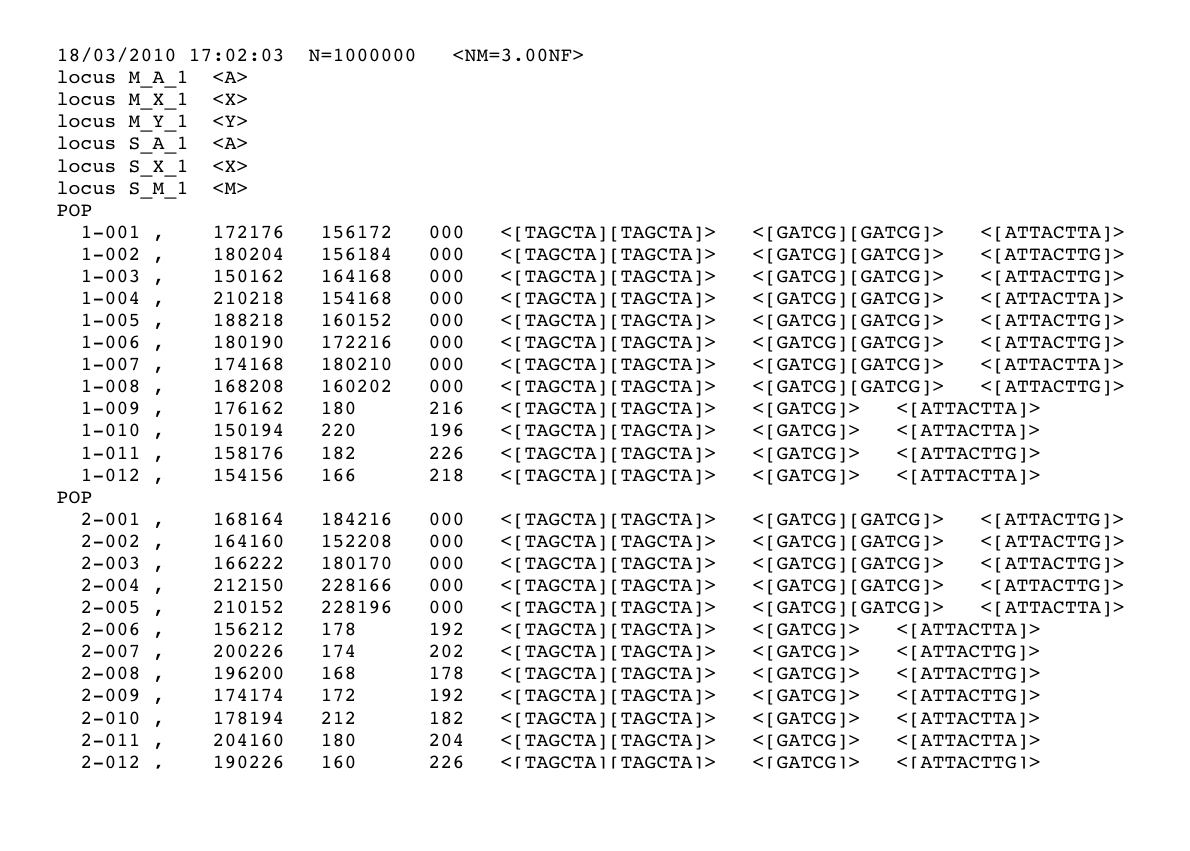
\includegraphics[scale=0.5]{gui_pictures/screenga001.png}
\end{figure}

In the second example, the species is haploid. Individuals have been genotyped at three autosomal microsatellite loci and one mitochondrial DNA sequence locus. The species being haploid (deduced from the presence of autosomal haploid loci), no indication of the sex-ratio appears in the title line.

\begin{figure}[h]
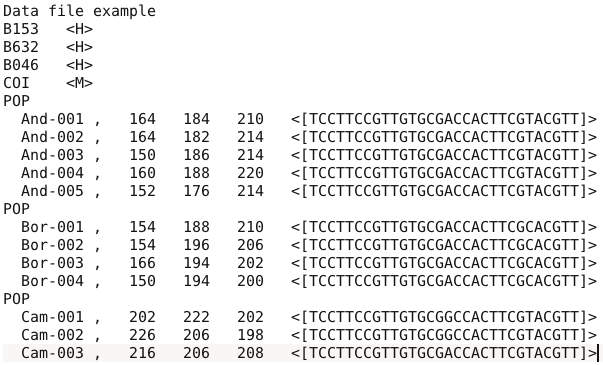
\includegraphics[scale=0.5]{gui_pictures/screenga002.png}
\end{figure}

In the third example, the species is diploid and has been genotyped at a large number of SNP autosomal loci. The first line provides the species sex-ratio. The second line indicates what's in the different columns : individual name in column 1, individual sex in column 2, population name in column 3 and one column per SNP locus. Columns are sparated by one or more spaces. SNP are coded 0, 1 or 2 according to the number of reference alleles. Only the top left part of the data file is represented below :

\begin{figure}[h]
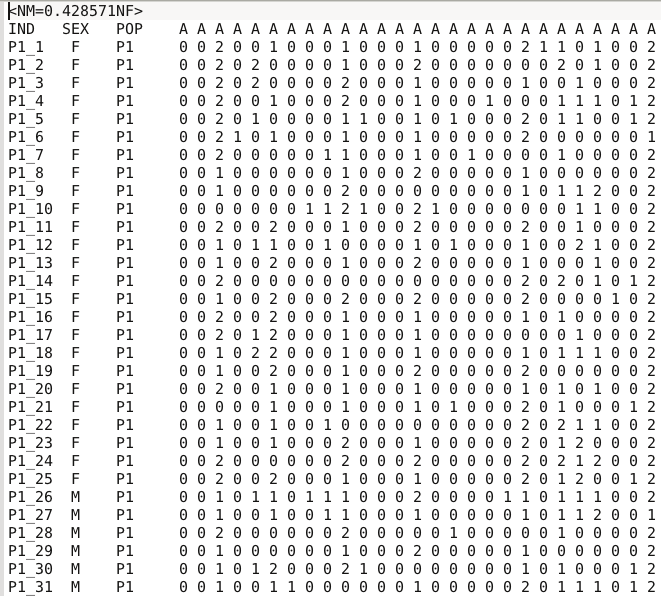
\includegraphics[scale=0.5]{gui_pictures/screenga003.png}
\end{figure}



\clearpage
\section{Cluster version}
The process of simulating data sets is generally a time consuming part of the ABC approach. Typically, one to several millions  data sets are needed to build up a reference table and this process can last several hours to several days. For those  that can have access to a computer grid cluster, two additional programs are available. They both run under Linux. Source files are written in Delphi pascal and can be compiled with Free Pascal Compiler (http://www.freepascal.org/download.var) using the command line :\\
\texttt{>fpc -Sd -m Delphi <filename>}
  \begin{description}
  \item[\texttt{diyabc\_sim}] :\\
  This program simulates a given number of data sets according to the information given in a \texttt{reftableHeader} file. The simulated data sets are output in a \texttt{reftable} file. This program requires 3 parameters : the name of the reftableHeader file, a string that will be affixed to the name of the reftable file (to distinguish it from other reftable files) and the number of desired simulated data sets. This programs has two input files : the reftableHeader file and the data file. The data file must match the one written at the beginning of the reftableHeader file. The data file is just needed to evaluate sample sizes and number of loci as well as determining missing data. As an example, supposing a reftableHeader file named \texttt{mydataanalysis.reftableHeader}, a command such as :\\
  \texttt{>diyabc\_sim mydataanalysis 01 5000}\\
  will produce a reference table file named \texttt{mydataanalysis01.reftable}  containing 5,000 simulated data sets according to the observed data set and analysis summarized in   \texttt{mydataanalysis.reftableHeader}. 
  
  \item[\texttt{diyabc\_cat}]:\\
  This program pools all reftable files of a directory into a single reftable file. This programs requires 2 parameters : the name of the reftableHeader file used to generate all the reftable files to be pooled and the name of the output reftable. \texttt{diyabc\_cat} reads the reftableHeader file (which has to be in the same directory), scans all available reftable files present in the directory and select all those with a header that matches the reftableHeader file.  The selected files are then copied to a single reftable file. Following with the example above, a command such as :\\
  \texttt{>diyabc\_cat mydataanalysis mda}\\
  will pool all reftable files with header matching \texttt{mydataanalysis.reftableHeader} in an output file named \texttt{mda.reftable}. 
  \end{description}
  
  The cluster is just used to produce a reftable file ready to be analyzed by DIYABC. All treatments are thus performed (under Windows) with the DIYABC programs. A typical session will include :\\
  \begin{enumerate}
  \item Using DIYABC, input data file name, provide scenario(s), provide priors for historico-demographic and mutationnal parameters, provide motif lengths and ranges, select summary statistics, simulate a few datasets (in one wants to check that the ouput is OK, but this last step is not compulsary). 
  \item Transfer the reftableHeader file and the data file on the cluster and using \texttt{diyabc\_sim} and \texttt{diyabc\_cat} as explained above, create a large reftable file.
  \item Transfer the reftable file back to the Windows directory where the analysis began and rerun DIYABC to perform comparison of scenarios, estimation of parameters or computation of bias/precision as needed.  
  \end{enumerate}
  For those who have access to a cluster with Sun's Grid Engine software, they can use the following script to create multiple reference tables (see next page). However, this script will not exempt the user to  manually run \texttt{diyabc\_cat} to concatenate all reference tables in a single one. The script is run with the following four parameters :\\
  
  \texttt{>ScriptABC file.dat file.reftableHeader n\_jobs n\_iter\_per\_job}
\clearpage
\begin{figure}
\caption{Bash script that can be run with Sun Grid Engine software}
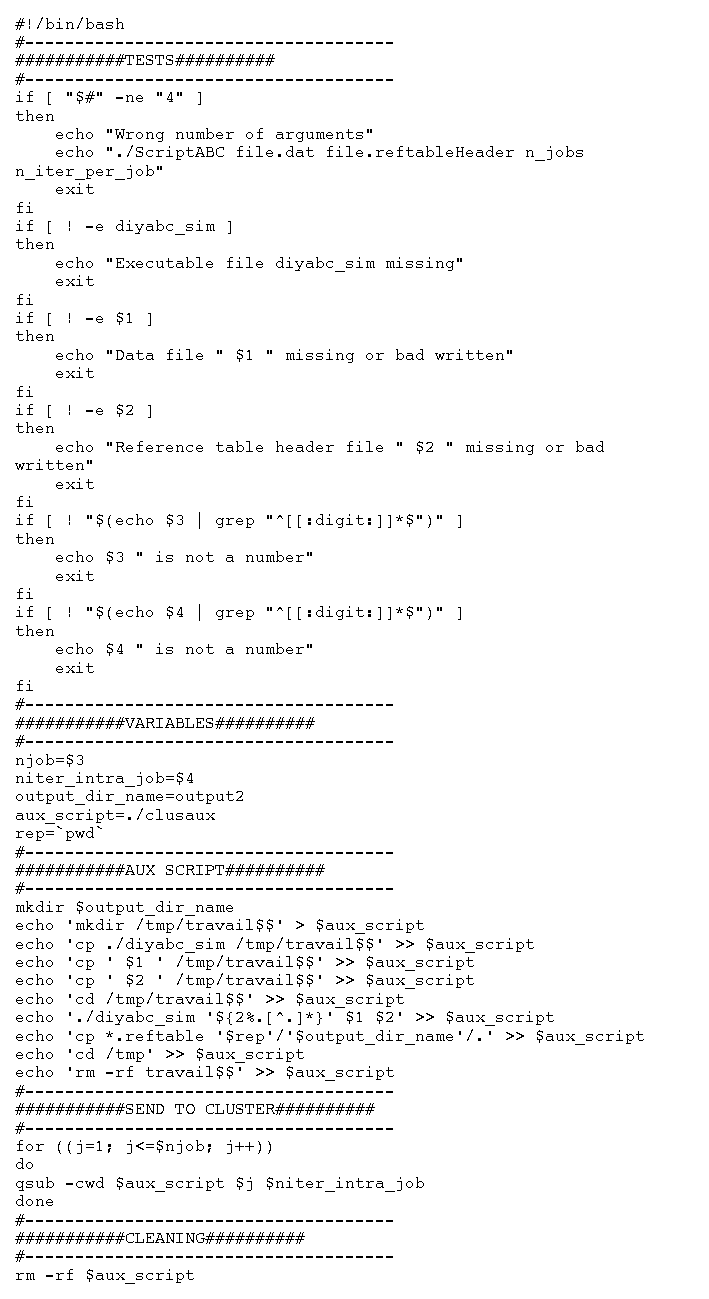
\includegraphics{gui_pictures/script_SGE.pdf}
\end{figure}

\clearpage
\subsection{A note about the random number generator used in DIYABC}

The random number generator used in DIYABC is of the \emph{Multiply With Carry} type invented by G. Marsaglia (see http://en.wikipedia.org/wiki/Multiply-with-carry for detailed explanations and references; see also http://www.rlmueller.net/MWC32.htm for a more condensed description).\\
The major interests of this random generator are :
\begin{itemize}
\item  it is very simple to program 
\item it is also very fast
\item there is a large choice of random number sequences among which to choose
\item the period of each sequence is a simple function of two parameters that define the sequence
\end{itemize} 

Four parameters define a unique sequence of pseudo random numbers. They are called the \emph{modulo} ($M$), the \emph{multiply}($m$), the \emph{initial x} ($x_0$) and the \emph{initial carry} ($c_0$). Only the last two parameters change when drawing a number, according to the following equations : \\

$x_i$ =$ [(m * x_{i-1} + c_{i-1}] $ \textsf{modulo} $M$\\  

$c_i$ = $[(m * x_{i-1} + c_{i-1}]$  \textsf{div}\footnote{\textsf{div} is the integer division, i.e. the result ($c_i$) is the integer part of the ratio.} $M$\\

In DIYABC, we chose a 24-bit generator, meaning that the \emph{modulo} parameter is fixed to $M$=$2^{24}$=16777216.\\
The \emph{multiply} parameter, which defines the sequence, is chosen among numbers that garanties a period larger than $10^{15}$. \\
The last two parameters, \emph{initial x and carry} are drawn at random, using the Delphi \textsf{random} function. \\

The multithreaded sections of the codes which require random draws are such that each thread uses its own random generator (defined by its own \emph{multiply} parameter). This solution spares writing conflicts from different threads since each call to a random generator involves writing new values of its $x$ and $carry$ parameters. 
The current version of DIYABC contains 10,000 possible values for this \emph{multiply} parameter (over the 43,701 possible). Since the number of threads is set equal to the number of cores, that should be enough for the moment.\\

\textbf{Important note for users of the cluster version}\\
Concerning the program \texttt{diyabc\_sim}, the Delphi \textsf{random} function has been replaced by reading bytes from the \texttt{/dev/random} file. However, when several jobs are sent to the same computer, the latter being multicore, there is a risk that these jobs read the same bytes and hence that they draw the same sequence of random numbers. To avoid this situation, the program uses the second parameter which is different among jobs to define the \emph{multiply} parameter of the sequence. Consequently, if the cluster contains multicore computers, it is strongly advised to use successive integers as second parameters for  \texttt{diyabc\_sim}. Furthermore, \texttt{diyabc\_sim} can use multiple threads. If one knows the number of cores of the computer on which the job will run, one can  add a fourth parameter equal to this core number. In that case, all cores will use the same \emph{multiply} parameter (defined by the second parameter if the latter is an integer), but different values of $x_0$ and $c_0$, because all the latter are now red sequentially from \texttt{/dev/random}.
 


  